\section{Impact on Speed and Position Control}

The compensator discussed up to this point is tightly coupled to the physical system and requires certain amplifier characteristics to be experimentally determined.
In order to simulate amplifier and motor non-linearities a lookup table method for linearizing the system was used.
The measured nonlinearities and compensator curves may be seen in figure \ref{fig:dataplots}.

\begin{figure}[ht]
    \centering
    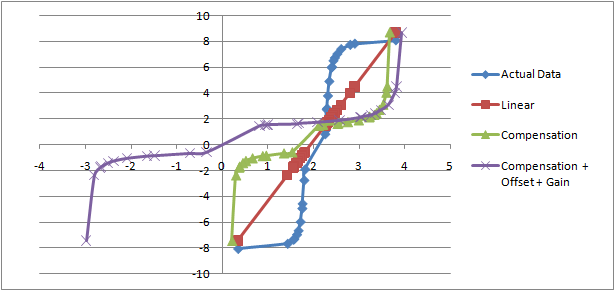
\includegraphics[width=.80\textwidth]{images/DataPlots.png}
    \caption{Amplifier Non-Linearities and Compensation Curves}
    \label{fig:dataplots}
\end{figure}


Position control and speed control experiments were performed using only the lookup table and repeated with lookup table and compensation curve.
Using only the lookup table (with no compensation) corresponds to the case of assuming amplifier linearities in the presence of non-linear characteristics.
When the lookup table and compensation curve were used together, they were seen to cancel and functionally appear not to exist.
This is due to the fact both lookup tables were created from the same set of data and perfectly canceled each other in the simulation.
Results for both experiments can be seen in figure \ref{fig:speedctrl} and figure \ref{fig:positionctrl}.

\begin{figure}[ht]
    \centering
    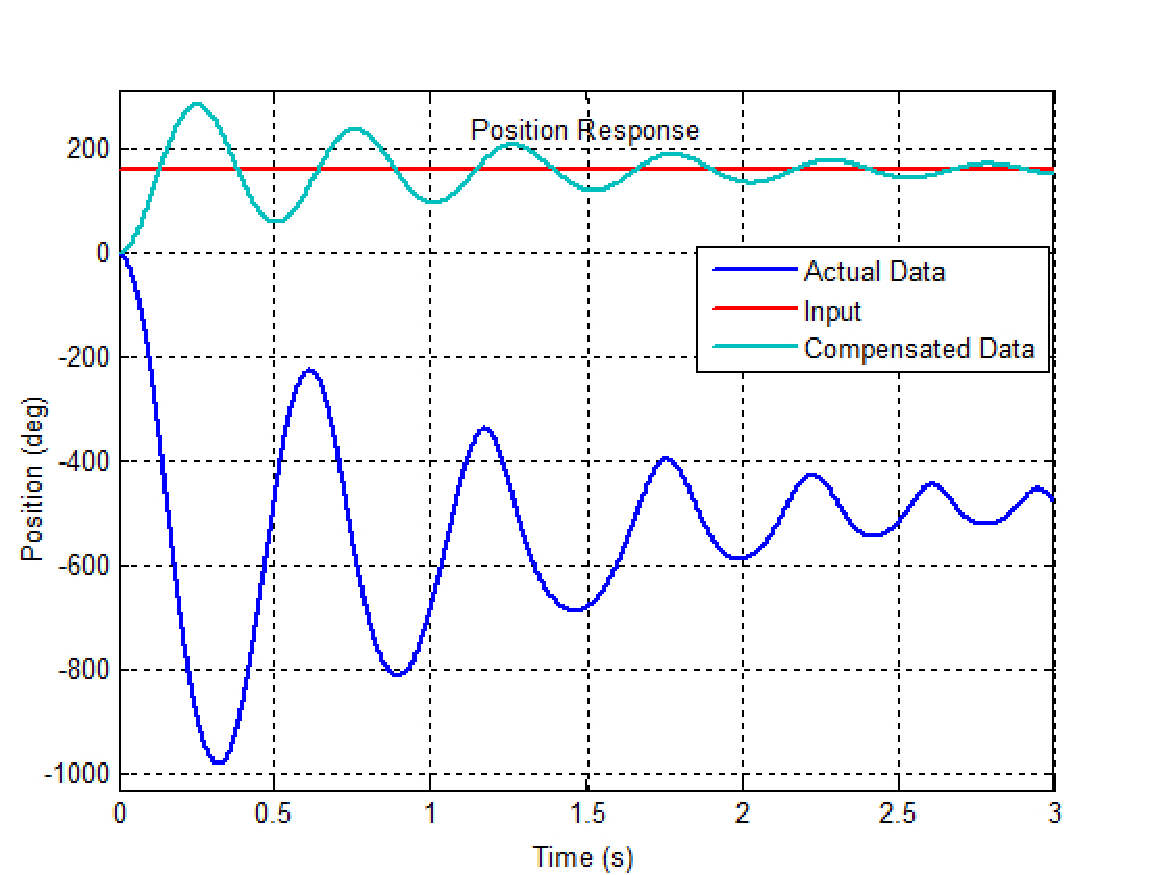
\includegraphics[width=.75\textwidth]{images/HW2position.pdf}
    \caption{Speed Control Experiment results}
    \label{fig:speedctrl}
\end{figure}

\begin{figure}[ht]
    \centering
    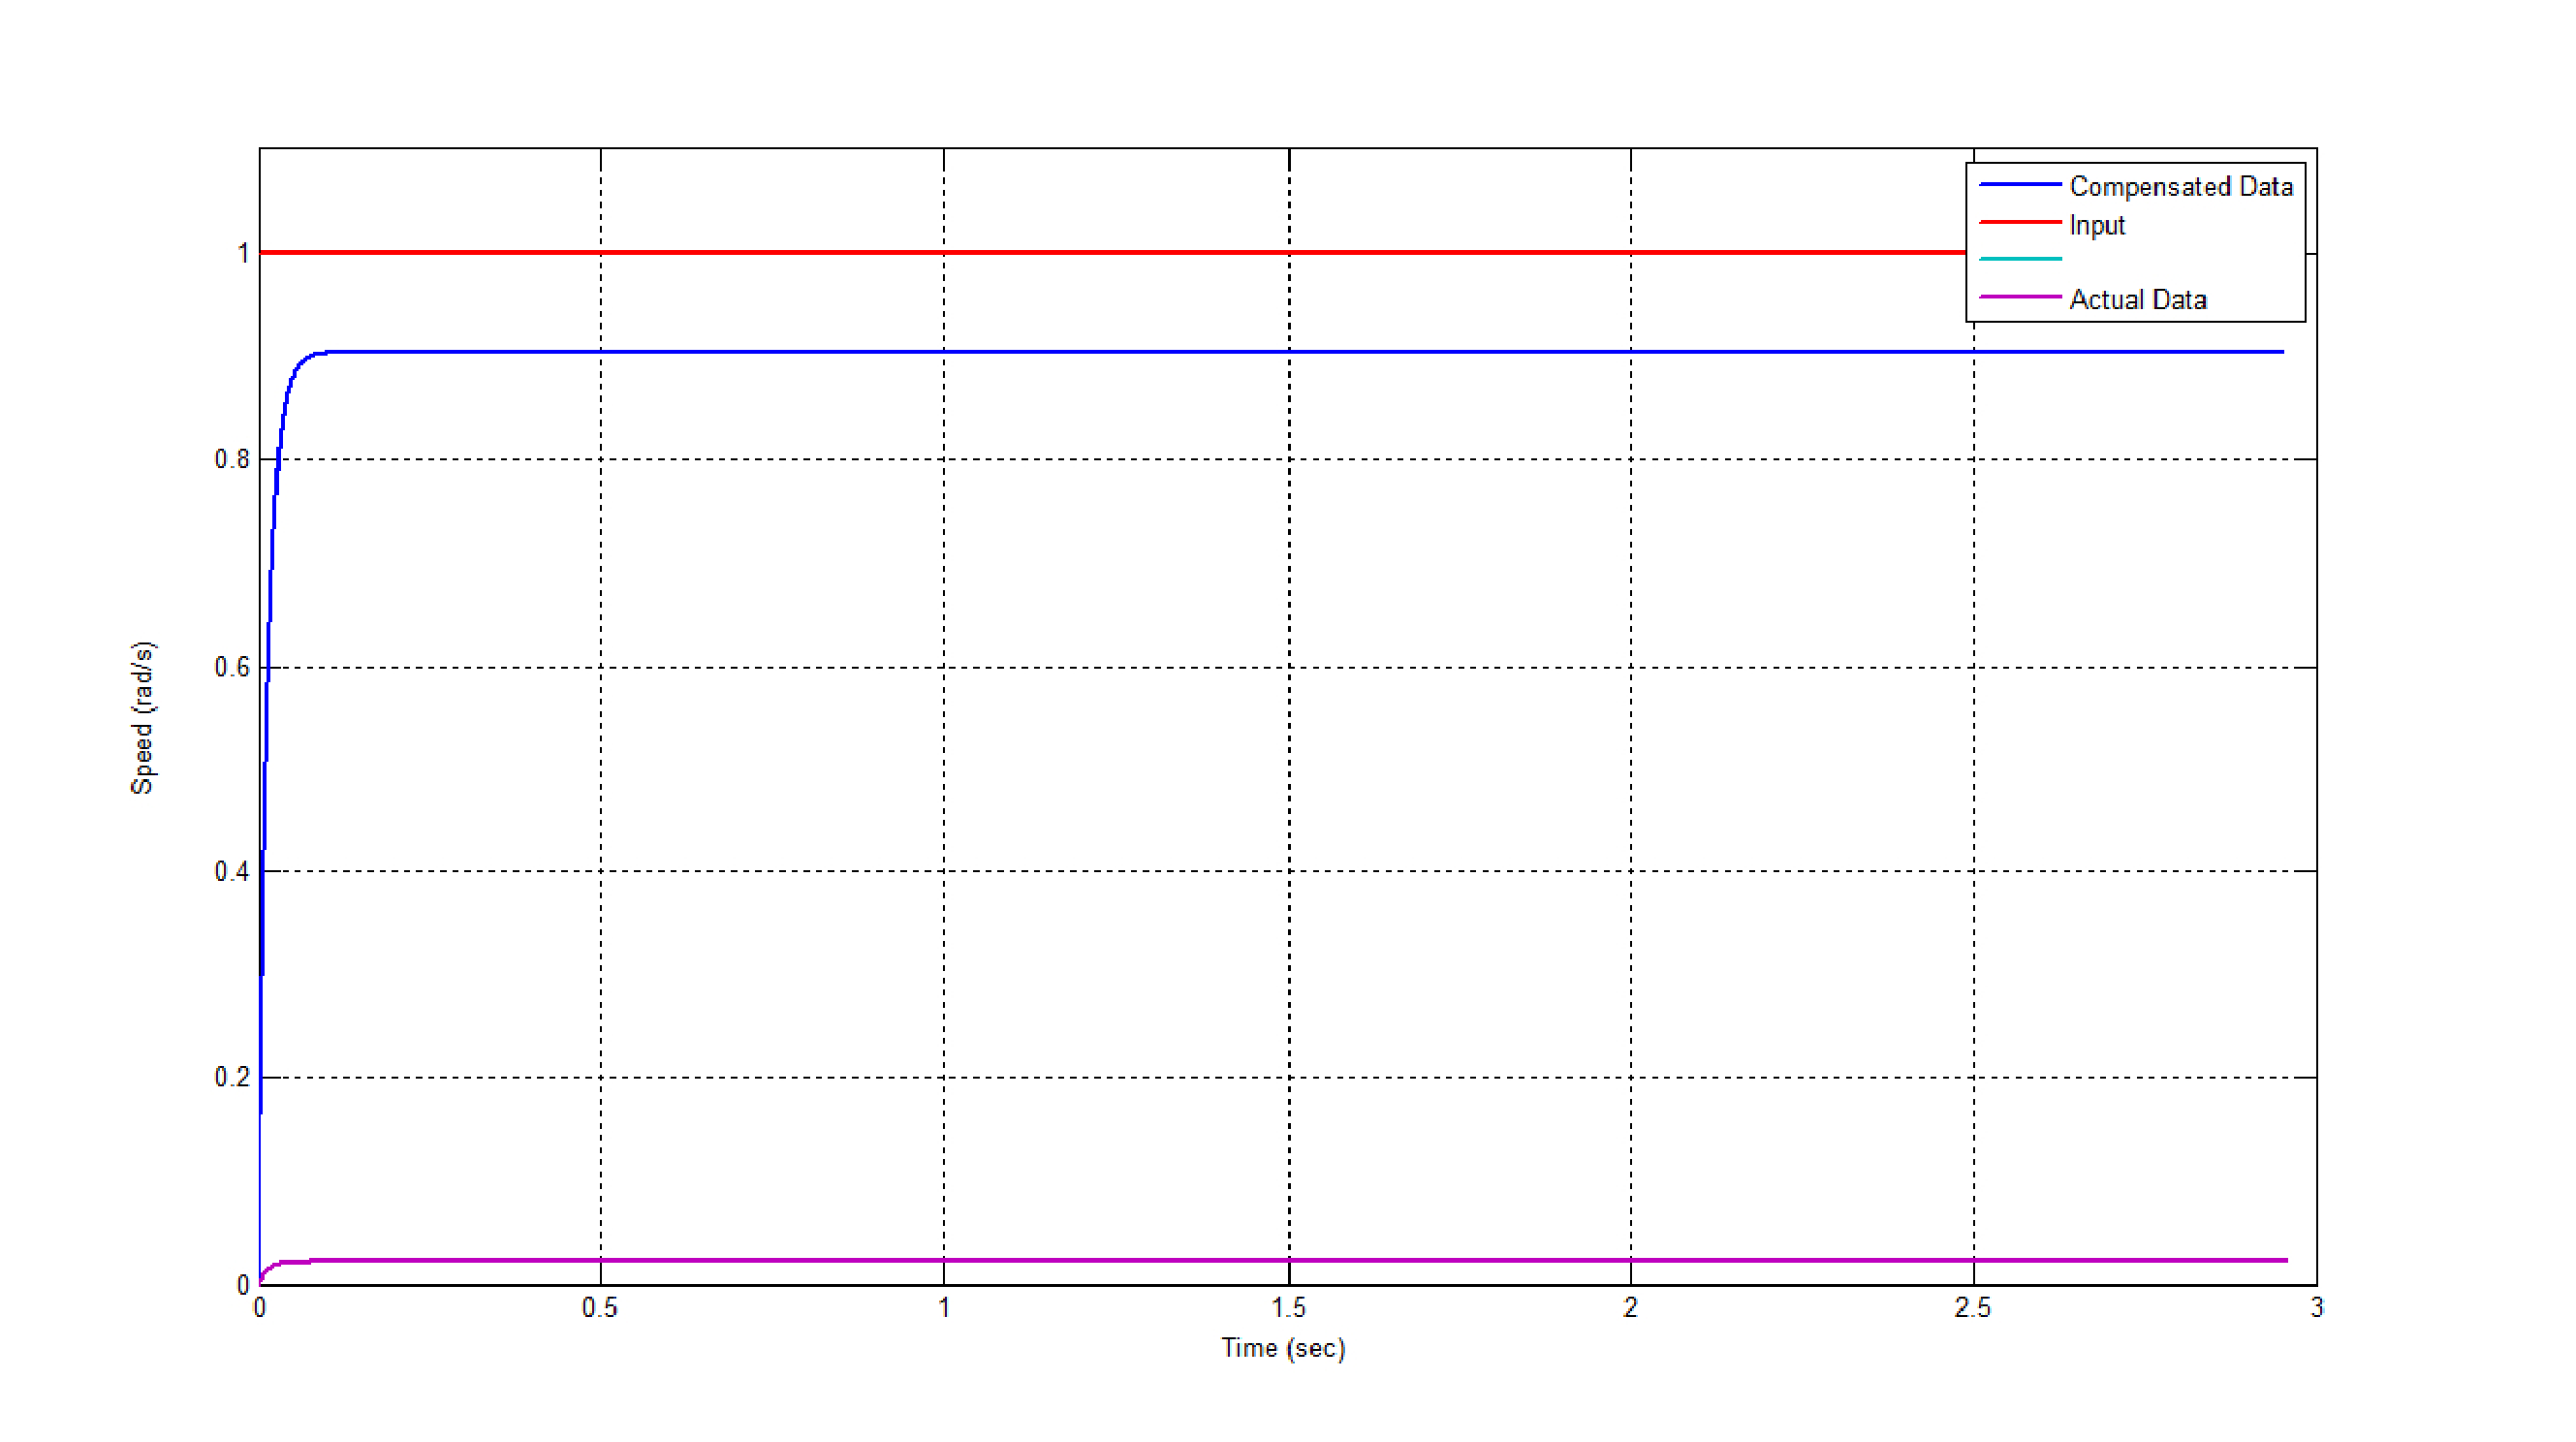
\includegraphics[width=.75\textwidth]{images/HW2speed.pdf}
    \caption{Position Control Experiment results}
    \label{fig:positionctrl}
\end{figure}